% \clearpage
\phantomsection
\chapter{Anexo de imágenes}
\label{chap:anexo_imagenes}

%\section{Imágenes del Proyecto Técnico}

    % Colores del diagrama: PFI, reserva de contingencia y proyección del producto
    \definecolor{ganttpfi}{HTML}{2E86AB}
    \definecolor{ganttreserva}{HTML}{BBBBBB}
    \definecolor{ganttproducto}{HTML}{E4572E}

    \begin{figure}[H] \centering
        \begin{ganttchart}[
                hgrid, vgrid,
                x unit = 0.78cm,
                y unit title = 0.6cm,
                y unit chart = 0.55cm,
                title/.append style = {fill=gray!15},
                title label font = \small\bfseries,
                bar label font = \small,
                group label font = \small\bfseries,
                milestone label font = \small\itshape,
                bar/.append style = {fill=ganttpfi, draw=none},
                bar height = 0.55,
                group/.append style = {fill=black!75},
                group height = 0.25,
                group peaks height = 0.15,
                group peaks width = 0.12,
                group left shift = 0,
                group right shift = 0,
                milestone/.append style = {fill=black!75},
                milestone height = 0.55,
            ]{1}{11}

            \gantttitle{PFI}{6} \gantttitle{Proyección del producto}{5} \\
            \gantttitlelist{1,...,11}{1} \\

            \ganttbar{Documentación y trazabilidad}{1}{10} \\

            \ganttgroup{Fase 1: datos y modelo}{1}{3} \\
            \ganttbar{Requisitos regulatorios}{1}{1} \\
            \ganttbar{Análisis exploratorio de datos}{1}{1} \\
            \ganttbar{Preprocesamiento de los datos}{1}{2} \\
            \ganttbar{Entrenamiento del modelo}{2}{3} \\
            \ganttbar{Evaluación e integración de Grad-CAM}{3}{3} \\
            \ganttbar{Solicitud de muestras locales}{1}{4} \\

            \ganttgroup{Fase 2: aplicación web}{3}{4} \\
            \ganttbar{\textit{Backend} (API con FastAPI)}{3}{4} \\
            \ganttbar{\textit{Frontend} (React)}{3}{4} \\
            \ganttbar{Usuarios y suscripción}{4}{4} \\
            \ganttbar{Despliegue en servidor VPS}{4}{4} \\
            \ganttmilestone{Prototipo terminado}{4} \\

            \ganttbar[bar/.append style={fill=ganttreserva}]{Reserva de contingencia}{5}{6} \\

            \ganttgroup{Fase 3: validación clínica}{7}{8} \\
            \ganttbar[bar/.append style={fill=ganttproducto}]{Evaluación con muestras locales}{7}{8} \\
            \ganttbar[bar/.append style={fill=ganttproducto}]{Pruebas de usabilidad}{8}{8} \\

            \ganttgroup{Fase 4: certificación y lanzamiento}{9}{10} \\
            \ganttbar[bar/.append style={fill=ganttproducto}]{Cierre del informe técnico}{9}{9} \\
            \ganttbar[bar/.append style={fill=ganttproducto}]{Inscripción ante la ANMAT}{9}{10} \\
            \ganttbar[bar/.append style={fill=ganttproducto}]{Documentación legal}{9}{10} \\
            \ganttbar[bar/.append style={fill=ganttproducto}]{Comunicación y manual de usuario}{10}{10} \\
            \ganttmilestone{Lanzamiento comercial}{10}

        \end{ganttchart}
        \caption{Diagrama de Gantt de las actividades del proyecto.}
        \label{fig:anexo_gantt}
    \end{figure}


%\section{Imágenes del Análisis de Producto de Mercado}

    \begin{landscape}
        \thispagestyle{empty}
        \begin{figure}[H] \centering
        
            \makebox[\linewidth][c]{\hspace*{1 cm}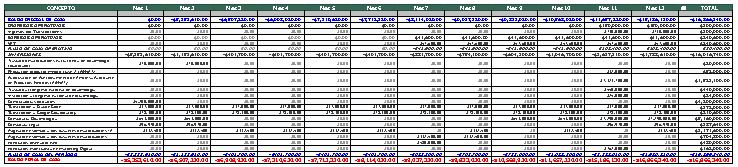
\includegraphics[height=0.39\textheight]{img/caja_desarrollo.pdf}}
            \caption{Flujo de caja correspondiente al desarrollo del proyecto (primer año).}
            \label{fig:anexo_caja_desarrollo}
            
            \makebox[\linewidth][c]{\hspace*{1 cm}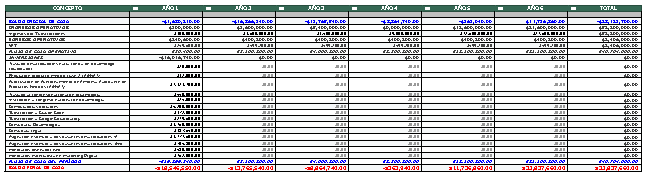
\includegraphics[height=0.45\textheight]{img/caja_años.pdf}}
            \caption{Flujo de caja correspondiente a los primeros seis años.}
            \label{fig:anexo_caja_años}
        \end{figure}
    \end{landscape}
